\newtheorem{theorem}{Theorem}[section]
\newtheorem{corollary}{Corollary}[theorem]
\newtheorem{lemma}[theorem]{Lemma}
\section{Notes for the reader}
This report has been written as a survey on random graphs and the different ways to approach them.
This section gives an overview of the structure of the report and different notations that are used in this report, all of the vocabulary introduced here will be properly defined in the following of this report.
\paragraph{Structure of the report}
It is structured in three different chapters, the first one is mostly an introduction to the language of graph theory followed by a very short introduction to what is a random graph.
The last part of the introduction is a proof of Cayley's formula, formula which is central in many enumerative proofs on random graphs.
\newline
The second chapter gives a description of the Erd\"os-R\'enyi model. 
Different techniques to solve graph problems are used, the theorem on connectivity and the stability number use enumerative techniques. 
The section on the diameter contains a long proof which is applied in the end using the probabilistic method which exhibits the existence of graphs satisfying certain properties.
The second chapter also contains a formal characterisation of graph properties and a theorem on the existence of thresholds for graph properties.
This chapter concludes with a generalisation of the Erd\"os-R\'enyi in which we consider that all edges do not necessarily have the same probability of appearance.
This allows us to finish the proof of connectivity and obtain a result on random bipartite graphs.
\newline
The third chapter is focused on the phase transition of random graphs and it uses many different exploration techniques.
The first part is on a formal definition of a Galton-Watson process and the probability of survival of such a process using martingales.
It also contains important results on the links between different kinds of Galton-Watson process and random graphs.
Then a study is done on the subcritical case using the Breadth-First search algorithm and a study of the supercritical case 
is done using the recent approach which uses the Depth-First search algorithm.
\newline
This report also contains an Appendix in which several results used in the report are detailed and most of them are proved.
\newline
In this report most of the results are proved and it is nearly self-contained.
However some results are admitted otherwise the report would have vastly exceeded the expected length.
\paragraph{Notations} The author has tried to be as close as possible from standard notations. 
Here some notations are presented, $\mathbb{P}, \mathbb{E}, \mathbb{V}$ respectively define a probability measure, the expectation and the variance.
$\mathcal{G}_n$ will denote a probability space of random graphs on $n$ vertices and $\mathbb{G}_n$ will be a random (graph) variable in a specified space of random graphs.
The distinction between $\mathcal{G}$ and $\mathbb{G}$ is not necessarily done.
We will say that a property is satisfied with high probability if its probability is tending to one as $n$ goes to infinity.
\section{Graph theory}
\footnote{ For a very simple introduction to graph theory, see \cite{Trudeau93}, for an advanced review of graph theory, see \cite{Bondy08}}
Formally a \emph{graph} $G$ is defined as $G = (V(G), E(G))$, with $V(G)$ denoting the vertex set (the points or nodes) of $G$ and $E(G)$ as $E(G) \subseteq \{ \{x, y\}, x, y, \in V(G), x \neq y \}$, the set of edges (the lines) of $G$. 
\newline
This is the simplest way to define a graph, hence this kind of graph is usually called a \emph{simple graph}. 
More general graphs can be defined, for instance the loopy graphs, multigraphs, directed graphs or hypergraphs. 
They are not of major importance in this report so they won't be detailed here, their formal definition can be found in almost any book on graph theory ( see for instance \cite{Bondy08} ).
\newline
We will call two vertices $u, v \in V(G)$ as \emph{adjacent} if $\{u, v\} \in E(G)$ and we will write it as $u \leftrightarrow v$. 
We may also refer to edges being adjacent if they share a vertex.
\newline
As an example of a graph we can consider the following graph with $ V(G) = \{a, b, c, d, e\}, E(G) = \{e_1,e_2, e_3, e_4, e_5, e_6, e_7\}$ for:
\begin{align*}
	e_1 = \{a, b\}\quad
	e_2 = \{a, c\}\quad
	e_3 = \{b, c\}\quad
	e_4 = \{a, d\}\\
	e_5 = \{c, d\}\quad
    	e_6 = \{a, e\}\quad
	e_7 = \{c, e\}
\end{align*}
\begin{figure}
	\centering
	\begin{tikzpicture}[scale=2]
		\tikzstyle{every node} = [node distance = 40cm]
		\Vertex{e}
		\NOEA(e){a}
		\SOEA(e){c}
		\NOEA(c){b}
		\EA(b){d}
		\Edge[label=$e_1$](a)(b)
		\Edge[label=$e_2$](a)(c)
		\Edge[label=$e_3$](b)(c)
		\tikzstyle{EdgeStyle}=[bend left]
		\Edge[label=$e_4$](a)(d)		
		\Edge[label=$e_7$](c)(e)
		\tikzstyle{EdgeStyle}=[bend right]
		\Edge[label=$e_5$](c)(d)
		\Edge[label=$e_6$](a)(e)	
	\end{tikzpicture}
	\caption{A graphical representation of $G$}
\end{figure}	
The \emph{adjacency matrix} of a graph $G$ is the $n \times n$ matrix defined as $A_G = (a_{u,v})$ with $a_{u, v} = \mathbbm{1}_{E(G)}(\{u, v\})$
\begin{equation}
	A_G = \kbordermatrix{
		  & a & b & c & d & e \\
		a & 0 & 1 & 1 & 1 & 1 \\ 
		b & 1 & 0 & 1 & 0 & 0 \\ 
		c & 1 & 1 & 0 & 0 & 1 \\ 
		d & 1 & 0 & 0 & 0 & 0 \\ 
		e & 1 & 0 & 1 & 0 & 0 \\ 
	}
\end{equation}

It is interesting to note that an adjacency matrix is real and Hermitian, thus all of its eigenvalues are real and the study of their distribution is a classical topic in graph theory.
\newline
An important property of graphs is the \emph{degree} of the vertices, so we will denote by $d_G(v)$ the number of edges incident with $v \in V(G)$.
Observing that each edge has two ends and that the degree of a vertex is the number of edges having this vertex as an end. We obtain :
\begin{equation}
	\sum_{v\in V(G)} d_G(v) = 2 |E(G)|
\end{equation}
We also call the degree sequence the non-increasing sequence of its vertex degrees.
And we can also define the two following notations that will be useful in the following of this report, $\delta(G)$ as the minimal degree of $G$ and $\Delta(G)$ as the maximal degree of $G$.
\newline
We define a \emph{path} on a graph as a sequence of edges being two by two adjacent. 
One of the most fundamental properties of graphs is the connectivity.
We will say that a graph is \emph{connected}, if there is a path connecting any two edges. 
In fact we will consider simple\footnote{ More generally, the use of the adjective \emph{simple} denotes that we study something without any loops or multi-edges}  paths because we are studying simple graphs.
It is clear that if a path exists it is always possible to extract a simple path from it.
There are two famous kinds of path, the \emph{Hamiltonian path}, it is a path that includes all vertices of $G$. Analogously, an \emph{Eulerian path} is a path in which all edges are used exactly once.
\newline
If $v$ is a vertex, we will write $N(v)$ the set of vertices adjacent to $v$ which are called the \emph{neighbours} of $v$.
From this definition we may observe that $d_G(v) = |N(v)|$ if $G$ is a graph without loops. 
And we will call a (connected) \emph{component} of a vertex the set of vertices that can be reached from this vertex. 
Then a connected graph is a graph with only one component.
\newline
Some interesting graphs to which we will often refer are the complete graph on $n$ vertices, denoted by $K_n$, and the complete bipartite graph $K_{n,m}$. 
\begin{figure}
	\subfloat[][]{
	\centering
	\begin{tikzpicture}
			\tikzstyle{LabelStyle}=[fill=white,sloped]
			\tikzstyle{EdgeStyle}=[]
			\SetVertexMath
			\grComplete[RA=1.5]{5}
	\end{tikzpicture}
	}
	\subfloat[][]{
		\centering
		\begin{tikzpicture}
			\tikzstyle{LabelStyle}=[fill=white,sloped]
			\tikzstyle{EdgeStyle}=[]
			\SetVertexMath
			\grCompleteBipartite[RA=2.5, RB=3, RS=3]{3}{3}
		\end{tikzpicture}
	}
	\caption{ (a) The complete graph $K_5$ and (b) the complete bipartite graph $K_{3,3}$.}
\end{figure}
A \emph{complete graph} is a graph in which for any vertex, the set of neighbours is the rest of the graph. 
A graph is \emph{bipartite} if its set of vertices can be partitioned in two subsets $X$ and $Y$ such that every edge has one end in $X$ and one in $Y$. 
The \emph{complete bipartite graph} is a bipartite graph such that for all $x \in X$ we have $N(x) = Y$. 
This implies the same condition on the vertices in $Y$.
We will also call a \emph{cycle}, of size $n \geq 3$, denoted $C_n$ a graph whose vertices can be arranged in a cyclic sequence in such a way that two vertices are adjacent if and only if they are consecutive in the sequence.

As there is usually no confusion possible we will denote $V = V(G)$ and $E =E(G)$. 


\section{Random graphs}
The study of random graphs is a flourishing area of mathematics since its founding papers have been published by Erd\H{o}s and Renyi between 1959 and 1963 (\cite{erdos59} \cite{erdos60} \cite{erdosconnect61} \cite{erdosevol61} \cite{erdos63}).
Since then a lot of work has been done on random graphs, most of the questions on the Erd\H{o}s-Renyi model have found satisfying answers, and the model being simplistic, many new models have been developed.
So we will use the very vague definition by Janson \cite{Janson14}.
\begin{definition}
	A \emph{random graph} is a graph where nodes, or edges, or both are selected by a random procedure.
\end{definition}
More formally, a random graph is a random variable on a space of graphs.
This means that when studying random graphs, we can not only change the distribution but also the space in which we sample.
\newline
Usually we make the choice of sampling on a space of graphs containing any graph with a specified number of vertices.
\footnote{This choices differs from what usually appear in the real-world where networks are grown through time, see \cite{CHKNS01} for a discussion on fundamental differences between grown random graphs and the static random graphs.}
Some restrictions on this space might be done, for instance by selecting graphs with each vertex of the same degree ($r$-regular random graphs), or with the degree sequence following a specific distribution (like the Newman-Strogatz-Watts model \cite{Newman01}, \cite{Newman02}).
Sometimes random graphs are developped in order to produce a sampling space matching  some particular phenomenom observed in real-world networks.

For instance in social networks, two persons having a friend in common are likely to be friends which in the vocabulary of graph theory indicates the presence of a triangle.
For this purpose was developped the Watts-Strogatz small world model \cite{WattsStrogatz98} which has a large enough number of triangle. 
\footnote{More formally, a positive density of triangles}
It also features a "small world" characteristic meaning that for most of the vertices there exists a path linking them which is small enough.
\newline

\section{Cayley's formula}
In this section we will prove an important result that will be used several times in crucial demonstrations in this report. 
Indeed it will give an exact result on the number of spanning trees, which are the building blocks of connected graphs. 
A \emph{tree} is a special case of graph structure that can be defined in several equivalent ways. 
For instance, a tree is a connected graph such that upon removal of any of its edges, it becomes disconnected, equivalently it is a connected and acyclic graph
\footnote{An acyclic graph is a graph that doesn't contain any cycle.}.
We say of a tree that it is \emph{spanning} on its vertex set.
\begin{theorem}[Cayley's formula]\label{cayley}
	We have
\begin{equation}
    t_n = n^{n-2}
\end{equation}
with $t_n$ the number of spanning trees of a given set of $n$ vertices.
\end{theorem}
\begin{figure}[h]
	\centering
	\begin{tikzpicture}
			\tikzstyle{every node} = [node distance = 40cm]
		\SetVertexMath
		\Vertex{a}
		\SOWE(a){b}
		\SOWE(b){e}
		
		\SO(a){c}

		\SOWE(c){f}
		\SOEA(c){h}
		\SO(c){g}
		
		\EA(a){i}
		\SOEA(a){d}
		
		\tikzstyle{EdgeStyle} = [post]
		\Edge[](a)(b)	
		\Edge[](b)(e)	
		\Edge[](a)(c)	
		\Edge[](c)(f)	
		\Edge[](c)(g)	
		\Edge[](c)(h)	
		\Edge[](a)(d)	
		
	\end{tikzpicture}
	\caption{An example of a directed tree spanning on the vertex set $\{a,b,c,d,e,f,g,h\}$ but not spanning on the whole set (which includes $i$).}
\end{figure}	
The proof will need to make use of directed trees.
More generally, we define \emph{directed graphs} as graphs \footnote{Often simply called digraphs (or ditrees).} in which the adjacency relation is not assumed to be symmetric
\footnote{In a directed graph an edge can only be followed in one direction.}.
We also define doubly rooted trees as trees with two special labels "Start" and "End" that can be attached to any vertices.
In such a tree, for any vertex, there exists a path to the vertex labelled "End"
\footnote{A tree with only the label "End" is called a \emph{rooted} tree, we observe that the corresponding directed tree is unique.}.
We will call "$SEL$" the vertices that are in the path from "Start" to "End". 
We also denote by $DRT_n$ the set of doubly rooted trees on $n$ vertices.
\newline
As a consequence of this definition we have $|DRT_n| = n^2 t_n$, with $|\ |$ denoting the cardinal. 
To prove the theorem it is then sufficient to prove that the number of elements in $DRT_n$ is equal to $n^n$.
We will base our approach on Joyal's proof \cite{joyal} and show a bijection between the set of doubly rooted trees on $n$ vertices and the set of functions from $\{1, 2, \ldots, n\}$ to $\{1, 2, \ldots, n\}$.
The presentation of the proof we use comes from \cite{JoyalProof}.
We recommend the reader to follow the proof using a given function as an example, see for instance Figure \ref{fig:exampleJoyal} which is the corresponding doubly rooted tree of the function defined in \eqref{eq:functionJoyal}.
\begin{proof}
We will use the notation $[n] = \{1, 2, ..., n\}$ and $V = [n]$.
Let's take $f:V \longrightarrow V$, and let's consider the directed graph of $f$. That is, $\forall v_1, v_2 \in V$ we have $v_1 \rightarrow v_2$ if and only if $f(v_1) = v_2$.
Drawing such a graph for any function, and it will appear two different kind of structures: directed lines leading to cycles, and cycles. 
Also, the whole graph will be a disjoint union of such components.
It can be interesting to observe the case in which $f$ is a permutation and then observe that the graph of $f$ is a union of disjoint cycles as expected from the common group theory result.
\newline
We now take $C \subseteq V$ the set of vertices that are part of a cycle under the action of $f$. Equivalently,
\begin{align*}
    C = \{ x : \exists i \geq 1 s. t. f^i(x) = x \}
\end{align*}
Let $k = |C|$ and write $C_<$ as $C_< = (c_1 < c_2 <...<c_k)$ the ordered set 
\footnote{The $c_i$ being integers we simply order them in increasing order.}
and now we will construct a graph with the vertex set $C = f(C)$, and the edge set $E = \bigcup_{i=1}^{k-1} f(c_i)f(c_{i+1})$. We now have $G=(C, E)$ as a line of $k$ vertices, and we will call $f(c_1)$ the "Start" and $f(c_k)$ the "End" which is an oriented graph.
\newline
Now we will just append to this line the set of vertices that are not in $G$. So we construct $\tilde{E} = \bigcup_{x \in V \backslash C} x f(x)$ and $\tilde{G} = (V, E\cup\tilde{E})$ is a (directed doubly rooted) tree as it doesn't contain any cycle by construction and is clearly connected. It's obviously directed and  doubly rooted.
We have now done the biggest part of the proof, that is, going from a function to a doubly rooted tree.
\newline
We will now take a doubly rooted tree and transform it in a function. From the definition of trees there is a unique "Start" to "End" ( SEL ) path.
\newline
For vertices not on the $SEL$, for instance some vertex $j$, we define $f(j)$ as the first neighbour on the $j$ to end line.
\newline
For vertices on the $SEL$, 
\begin{align}
	SEL = (x_1, x_2, ..., x_k), \text{ and } SEL_< = (x_{\sigma_1}, x_{\sigma_2}, ..., x_{\sigma_k}) 
\end{align}
we define $f(x_{\sigma_i}) = x_i, \forall i \in [k]$.
\newline
Thus, we have two injective constructions, if composed give the identity, hence we have a bijection between the set of endomorphism of $[n]$ and the space of doubly rooted trees on $n$ vertices. So the proof is complete.
\end{proof}
\paragraph{An example}
We will here illustrate the proof using an example of a transformation from a function to a doubly rooted tree using the following function:
\begin{equation}\label{eq:functionJoyal}
	\begin{pmatrix}
			1 & 2 & 3 & 4 & 5 & 6 & 7 & 8 \\
			3 & 1 & 1 & 6 & 7 & 5 & 4 & 4
	\end{pmatrix}.
\end{equation}
The corresponding doubly rooted tree is then:
\begin{figure}[h]
	\centering
	\begin{tikzpicture}[]
		\Vertex[x=-3, y=0]{3}
		\Vertex[x=-1, y=0]{1}
		\Vertex[x=1, y=0]{6}
		\Vertex[x=3, y=0]{5}
		\Vertex[x=5, y=0]{7}
		\Vertex[x=7, y=0]{4}
		\Vertex[x=-1, y=-1.5]{2}
		\Vertex[x=7, y=1.5]{8}
		\tikzstyle{EdgeStyle}=[post]	
		\Edge[](3)(1)
		\Edge[](1)(6)
		\Edge[](6)(5)
		\Edge[](5)(7)
		\Edge[](7)(4)
		\Edge[](2)(1)
		\Edge[](8)(4)
	\end{tikzpicture}
	\caption{The corresponding doubly-rooted tree of \eqref{eq:functionJoyal}, the "Start" root is vertex 3, the "End" root is vertex 4.}
	\label{fig:exampleJoyal}

\end{figure}

